\subsection{Problem}
\renewcommand{\theequation}{\theenumi}
\begin{enumerate}[label=\thesection.\arabic*.,ref=\thesection.\theenumi]
\numberwithin{equation}{enumi}
\item Find the area of the triangle having vertices 
\begin{multline}
	\vec{A} = \myvec{1\\1\\1}\quad
	\vec{B} = \myvec{1\\2\\3}\quad
	\vec{C} = \myvec{2\\3\\1}
\end{multline}
	The following python code computes the area of $\triangle$ABC in Fig.\ref{fig:qone}.
	\begin{lstlisting}
	./codes/triangle/q1.py
	\end{lstlisting}
	\solution The area of $\triangle$ABC is defined as
	\begin{align}
		\frac{1}{2}\norm{\brak{\vec{B-A}} \times \brak{\vec{C-A}}}
	\end{align}
	\begin{figure}[!ht]
	\centering
	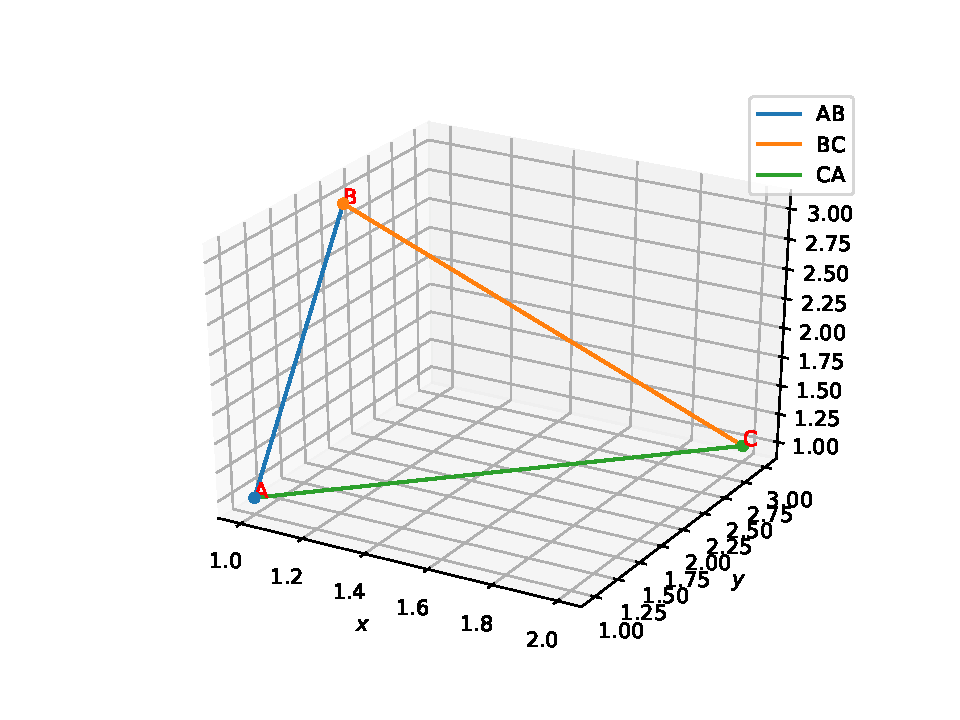
\includegraphics[width=\columnwidth]{./figs/triangle/q1.pdf}
	\caption{Triangle of Q.1.1.5}
	\label{fig:qone}	
	\end{figure}
	which is calculated and found as 2.29
\end{enumerate}

